%%%%%%%%%%%%%%%%%%%%%%%%%%%%%%%%%%%%%%%%%%%%%%%%%%
%% Bachelor's & Master's Thesis Template        %%
%% Copyleft by Dawid Weiss & Marta Szachniuk    %%
%% Faculty of Computing and Telecommunication   %%
%% Poznan University of Technology, 2020        %%
%%%%%%%%%%%%%%%%%%%%%%%%%%%%%%%%%%%%%%%%%%%%%%%%%%


% Szkielet dla pracy licencjackiej pisanej w języku polskim.

\documentclass[polish,bachelor,a4paper,oneside]{ppfcmthesis}


\usepackage[utf8]{inputenc}
\usepackage[OT4]{fontenc}
\usepackage{listings}
\usepackage{xcolor}
\usepackage{float}
\let\lll\undefined  % Usunięcie istniejącej definicji komendy \lll
\usepackage{amssymb}  % Załadowanie pakietu amssymb
\usepackage{amsmath}
\usepackage{longtable}
\usepackage{tikz}
\let\lll\undefined  % Usunięcie istniejącej definicji komendy \lll
\usepackage{amssymb}  % Załadowanie pakietu amssymb
\newtheorem{definition}{Definicja}[section]
\lstset{
  language=,
  basicstyle=\ttfamily\footnotesize,
  keywordstyle=\color{blue},
  commentstyle=\color{green},
  stringstyle=\color{red},
  showstringspaces=false,
}

%--------------------------------------
% Strona tytułowa
%--------------------------------------

% Autorzy pracy, jeśli jest ich więcej niż jeden
% wstaw między nimi separator \and
\author{%
   Paweł Błoch \album{145375} 
}
\authortitle{}                                % Do not change.

\title{Zastosowanie uczenia ze wzmocnieniem w zadaniu weryfikacji modelowej}

% Your supervisor comes here.
\ppsupervisor{r Iwo Błądek} 

% Year of final submission (not graduation!)
\ppyear{2024}                                 


\begin{document}

% Front matter starts here
\frontmatter\pagestyle{empty}%
\maketitle\cleardoublepage%

%--------------------------------------
% Miejsce na kartę pracy dyplomowej
%--------------------------------------

\thispagestyle{empty}\vspace*{\fill}%
\begin{center}Tutaj będzie karta pracy dyplomowej;\\oryginał wstawiamy do wersji dla archiwum PP, w pozostałych kopiach wstawiamy ksero.\end{center}%
\vfill\cleardoublepage%

%--------------------------------------
% Spis treści
%--------------------------------------

\pagenumbering{Roman}\pagestyle{ppfcmthesis}%
\tableofcontents* 
\cleardoublepage % Zaczynamy od nieparzystej strony

%--------------------------------------
% Rozdziały
%--------------------------------------

%Najwygodniej jeśli każdy rozdział znajduje się w oddzielnym pliku
\mainmatter%

\chapter{Wstęp}

% Wstęp do pracy powinien zawierać następujące elementy:
% \begin{itemize}
%     \item krótkie uzasadnienie podjęcia tematu; 
%     \item cel pracy (patrz niżej); 
%     \item zakres (przedmiotowy, podmiotowy, czasowy) wyjaśniający, w jakim rozmiarze praca będzie realizowana; 
%     \item ewentualne hipotezy, które autor zamierza sprawdzić lub udowodnić; 
%     \item krótką charakterystykę źródeł, zwłaszcza literaturowych; 
%     \item układ pracy (patrz niżej), czyli zwięzłą charakterystykę zawartości poszczególnych rozdziałów; 
%     \item ewentualne uwagi dotyczące realizacji tematu pracy np.~trudności, które pojawiły się w trakcie 
%     realizacji poszczególnych zadań, uwagi dotyczące wykorzystywanego sprzętu, współpraca z firmami zewnętrznymi. 
% \end{itemize}

Gałaź nauki zajmujące się "Model Checking" to obecnie bardzo szybko rozwijająca się gałąź nauki.
Jest to spowodowane licznymi zastosowaniami w których można skorzystać z narzędzii które dostarcza 
werfikacji modeli. Obecnie zastosowania jakie możemy znaleźć między innymi to
\begin{itemize}
    \item gry planszowe  ~\cite{Schlingloff}% Modeling and Analysis of Board Games
    \item planowanie misji dla autonomicznych agentów ~\cite{Gu}
    \item analiza i dowodzenia poprawności kodów źródłowych  ~\cite{Amazon}.
\end{itemize}

Celem który przyświecał podczas tworzenia tej pracy była próba stworzenia alternatywnych sposobów werfikacji 
modeli, skuteczniejszych od tych obecnie istniejących i wyznaczającyh standardy. Laureatka Nagrody 
Nobla Françoise Barré-Sinoussi w dziedzinie medycny powiedziała
\begin{quote}
    We are not making science for science. We are making science for the benefit of humanity.
    \end{quote}


Ciekawym obszarem jest analiza i dowodzenie poprawności kodów programistycznych. Zwłaszcza w obecnych czasach
gdy ilość kodu wytrzwarzana przez progmiastów z całego świata jest bardzo duża. Rok do roku liczba projektów programistycznych
rozpoczętych przez programistów wzrasta w dynamicznym tempie. Jednym z powodów jest pojawienie się ostatio
 modeli sztucznej inteligencji potrafiących
automatycznie generować oraz odpowiadać na pytania. Więcej o statystykach można poczytać w  ~\cite{Github}.

W tej pracy główny nacisk został położony na anlizę gier planszowych. Będziemy próbowali odpowiedzieć 
na pytanie czy i w jakim zakresie algorytmy uczenia ze wzmocnienieum i/lub algorytmy heurystyczne są w stanie 
polepszyć narzędzie typu "model checker". Narzędzie te umożliwiają automatyczną werfikację modeli.
Narzędzie te przyjmują na wejściu parę składającą się z modelu oraz formuły która będzie badana dla danego modelu.
Obecnie istnieje kilka tego typu narzędzi których opis znajdzie się w dalszej cześci pracy.

% \end{quote}



\chapter{Podstawy teoretyczne}
\subsection{Logika}
Aby mówić o werfikacji modeli musimy się wyposażyć w  elementarz teoretyczny. Potrzebne nam są podstawowe 
definicje i pojęcia zanim zaczniemy mówić o skomplikowanych modelach. Ważne jest również 
wprowadzenie i usystematyzowanie informacji z różnych źródeł. Rodział ten został oparty 
na świetnej książce ~\cite{Jamroga} i będzie stanowił fundament dalszej tej pracy.
Podstawowe elementy logiki można znaleźć w świetnej książce ~\cite[Podstawy Logiki]{batog1994podstawy} do której serdecznie
odsyłam.

 System wieloagentowy (ang. multi-agent system, MAS) to system składający się z autonomicznych podmiotów, działających 
 w tym samym środowisku. Jest on wykorzystywany do modelowania i opisywania systemów z którymi 
 spotykamy się w świecie informatyki i nie tylko. Agenci mogą podejmować akcje w jednym 
środowisku. Przykładem takiego środowiska mogą być wybory, gdzie grupa $n$ wyborców 
(agentów) bierze udział w procesie wyborczym.

Logika modalna którą będziemy się posługiwali jest rozszerzeniem klasycznej logiki 
o nowe operatory $\Box$ i konieczności $\diamond$. Formuła $\Box \phi$ oznacz, że $\phi$ 
jest prawdziwa zawsze w każdym stanie. Formuła $\diamond \phi$ oznacza, że $\phi$ jest prawdziwe 
w pewnym stanie. Spełniona jest przy tym zasada 
\begin{equation*}
    \lozenge \varphi \iff \neg \Box \neg \varphi
\end{equation*}

Wprowdzaimy teraz definicję modele Kripkiego.
\begin{definition}[Model Kripkiego]
    Niech \( PV = p, p', p'', \ldots \) będzie zbiorem zmiennych 
    zdaniowych. Modele logiki modalnej nazywane są modelami Kripkego lub modelami możliwych 
    światów i obejmują zbiór możliwych światów (lub stanów) \( St \),
     modalną relację dostępności \( R \subseteq St \times St \) oraz interpretację 
     zmiennych \( \mathcal{V} : PV \rightarrow 2^{St} \).
\end{definition}

Jeśli trójka $M=(St,R,V)$ będzie modelem kripkiego i $q$ będzie możliwym słowem w $M$,
to prawdziwość formuły $M,q$ jest dana relacją $ \models $ i jest zdefiniowana indukcyjnie 
przez zasady
\[
\begin{array}{ll}
M, q \models p & \text{wtedy i tylko wtedy, gdy} \quad q \in V(p), \quad \text{dla} \quad p \in \mathcal{PV}; \\
M, q \models \neg \varphi & \text{wtedy i tylko wtedy, gdy} \quad \text{nie} \quad M, q \models \varphi \quad (\text{często pisane} \quad M, q \not\models \varphi); \\
M, q \models \varphi \land \psi & \text{wtedy i tylko wtedy, gdy} \quad M, q \models \varphi \quad \text{i} \quad M, q \models \psi; \\
M, q \models \varphi \lor \psi & \text{wtedy i tylko wtedy, gdy} \quad M, q \models \varphi \quad \text{lub} \quad M, q \models \psi; \\
M, q \models \Box \varphi & \text{wtedy i tylko wtedy, gdy} \quad \text{dla każdego} \quad q' \in St \quad \text{takiego, że} \quad q R q', \quad \text{mamy} \quad M, q' \models \varphi; \\
M, q \models \Diamond \varphi & \text{wtedy i tylko wtedy, gdy} \quad \text{dla pewnego} \quad q' \in St \quad \text{takiego, że} \quad q R q', \quad \text{mamy} \quad M, q' \models \varphi.
\end{array}
\]

Prosty przykład modelu Kripkiego może wyglądać tak:


\subsection{Uczenie ze wzmocnieniem}
Uczenie ze wzmocnieniem to dynamicznie rozwijająca się część sztucznej inteligencji.
Jest to proces, w którym agent ucz się jakie działania podejmować w środowisku, 
aby uzyskać jak największą nagrodę. Agent uczy się w pewien sposób metodą prób i błędów,
nie jest dla niego jasne które akcje przyniosą mu największe nagrody. Problemy ten 
charakterysuje się opóźnioną nagrodą. Oznacza to, że za akcję podjęte w pewnym momencie 
wpływają nie tylko na bieżącę nagrody, ale również na przyszłe stany i nagrody z nimi związane.

Uczenie ze wzmocnieniem samo w sobie jest szerokim zagadnieniem, zawiera w sobie zarówno sam problem,
klasę metod którą są w stanie rozwiązać problem jak i całą dziedzinę nauki. Kluczowym aspektem 
jest rozróżnienie pomiędzy problemem a metodami służącymi do jego rozwiązania.

Problemy uczenia ze wzmocnieniem formalizujemy za pomocą procesów decyzyjnych Markova.
Agent musi w pewien sposób odczuwać stan środowiska, podejmować działania wpływające na środowisko 
i mieć cele związane ze stanem środowiska. Procesy decyzyjne Markova uwzględniają te trzy aspekty.

Uczenie ze wzmocnieniem rózni się od dobrze znanego uczenia nadzorowanego, w którym system uczy 
się bazując na podstawie poetykietownych przez nadzorcę przykładów ze zbioru uczącego.
Różni się również od uczenia nienadzorowanego, które zazwyczaj polega na znajdowaniu 
struktur i wzorców w nieoznaczonych zbiorach danych. Uczenie ze wzmocnieniem dąży 
uzyskania jak największej nagrody, a nie do odrykwania struktur w zbiorach danych.

Jednym z wyzwań przed którym stajemy wykorzystując uczenie ze wzmocnieniem jest przetarg 
pomiędzy eksploracją i eksplatacją. Agent musi wybierać pomiędzy akcjami, które przyniosły mu już 
nagrodę, a wybieraniem nowych akcjii i stanów których jeszcze nie zna, a te mogą mu przynieść 
nagrody w przyszłości. Ani eksplatacją ani eksploracja nie mogą być wykonywane wyłącznie,
gdyż uniemożliwi to agentowi uzsykanie celu.

\subsection{Algorytmy uczenie ze wzmocnieniem}
Podczas badań zostały wykorzystane różne algorytmy uczenia ze wzmocnieniem. Poniżej zostanie dokonana
ich krótka charakterystyka.

\subsection*{AlphaZero}
Algorytm AlphaZero jest zaawansowany algorytmem uczenia ze wzmocnieniem. Zmień on sposób myślenia 
w tej gałęzi nauki. Pokazał on, że sztuczna inteligencja jest w stanie osiągnąć poziom nie możliwy do 
osiągnięcia dla człowieka w grach planszowych dla dwóch graczy. W artykule ~\cite{alpha_zero} zaprezentowane
zostałe osiągnięcia dla dobrze znanych gier jak szachy, shogi czy go. Algorytm ten nauczył się grać bez 
wiedzy dziedzinowej. Proces nauki polega na grze z samym sobą, co stopniowo prowadzi do polepszania 
swoich umiejętności. AlphaZero składa się z kilku kluczowych elementów.

Głęboka sieć nueronowa ocenia pozycję na planszy, prognozuje prawodopodobieństwa wykonania ruchu i ocenia wynik gry.
Sieć możemy oznaczyć jako $(p,v)=f_{\theta}(s)$. Parametry $\theta$ to parametry sieci, $s$ to stan gry przyjmowany na wejście,
a wynikiem działania sieci jest wektor prawdopodobieństwa $p$ oznaczający prawdopodobieństwo wykonania ruchów oraz 
wartość oczekiwaną pozycji $v$.

Klasyczny algorytm przeszukiwania drzewa \textit{alfa-beta} został zastąpiony przez \textit{Monte Carlo Tree Search (MCTS)}
który jest bardziej ogólnym podejściem. Każda symulacja w MCTS wybiera ruchy na podstawie małej liczby odwiedzin (ruchów dotychczas mało eksplorowanych),
 wysokiego prawdopodobieństwa ruchu i wysokiej wartości stanu.

 Parametry $\theta$ sieci neuronowej są aktualizowane na podstawie wyników rozegranych gier oraz różnicy pomiędzy 
 przewidywanym wynikiem $v$ a rzeczywistym wynikiem gry. Minimalizowana jest minimalizacja funkcji straty, która składa 
 się z błędu średniokwadratowego i straty entropii krzyżowej 
 \begin{equation*}
    l = (z-v)^{2} - \sum_{a} p_{a} \log{q_{a} + c ||\theta||^{2}}
 \end{equation*}
 gdzie $c$ jest parametrem regularyzacji $L2$.

 Alphazero rozpoczyna proces treningu od losowych ruchów bez posiadania wiedzy domenowej oprócz reguł gry. Wraz z procesem 
 treningu AlphaZero zwiększa swoje umięjętności wskutek aktualizacji wag modelu. Algorytm ten jest algorytmem który bardzo szybko 
 się uczy. Dowodzi tego fakt, że zaledwie po czterech godzinach treningu model był w stanie pokonać dotychczas najlepszy 
 silnik szachowy \textit{Stockfish}

\chapter{Rozwinięcie}

\section{Wprowadzenie do problemu}
Celem tej sekcji jest porównanie werfikacji modelowej i technik uczenia ze wzmocnieniem w konteście analizy 
modeli reprezentujących grę dla dwóch graczy. Przeanalizujemy znaną grę Kółko i Krzyżyk. Analiza będzie polegała na wykonaniu dwóch eksperymentów. Pierwszym w nich będzie 
zamodelowanie gry jako modelu logicznego. Zostanie to wykonane i opisane w formacie \textit{ Interpreted Systems Programming Language
(ISPL)}. Po zamodelowaniu będzie konstruowali formuły do sprawdzenia przez model checker \textbf{MCMAS} które będą 
odpowiadały problemowi znajdowania strategii wygrywającej dla jednego z graczy. Będziemy zaczynali w pewnej pozycji,
początkowej lub planszą częściowo zajętą. Pytanie o strategię wygrywającą, jest równoznaczne z pytaniem 
czy istnieje strategia dla danego gracza która niezależnie od strategii drugiego gracza doprowadzi go do zwycięstwa.
Będziemy również wykorzystywali algorytmy uczenia ze wzmocnieniem do nauki modelu gry. Następnie będziemy rozgrywali 
gry pomiędzy nauczonymi agentami (lub losowymi) i na podstawie serii wyników będzie stawiali hipotezę co do prawdziwości 
danej formuły.

Wybór gry kółko krzyżyk jako pierwszego środowiska jest umotywowany kilkoma aspektami. Gra kółko krzyżyk 
jest znane praktycznie każdemu i to sprawia, że próg wejścia jest niski. Co więcej każdy czytelnik zrozumie 
zagadnienie które będziemy omawiali. Sama gra pozostaje cały czas interesującym tematem badań i opracowań.
Możemy je znaleźć między innymi w ~\cite{Deepa}, ~\cite{Dalffa2019-DALTLU}, ~\cite{Fogel}.
Gra jest cały czas problemem otwartym. Dokładniej mówiąc, otwarty jest problem dowiedzenia czy istnieje 
strategię wygrywającą dla gier o różnym rozmiarze. Jak podaje ~\cite{beck2008combinatorial} nadal otwartym problemem 
pozostaje gra $5 \times 5 \times 5$. Dowiedzione zostałe strategie dla gier $3\times 3 \times 3$ oraz 
$4 \times 4 \times 4$. W obu tych grach istnieje strategia wygrywająca dla graczy rozpoczynających rozgrywkę.
Dla gry $5 \times 5 \times 5$ przypuszcza się, że będzie to gra remisowa.
\subsection{Model checker STV}
Narzędzi \textit{stv} ~\cite{jamroga_stv} to jedno z najlepszych dostępnych narzędzi do werfikacji modelowej.
Jego współautorem jest polski naukowiec prof. dr hab. Wojciech Jamroga. Zalicza się on do grona najlepszych ekspertów w tej 
tematyce. Jest on również autorem wielu publikacji z tego zakresu. Narzędzi \textit{stv} posłuży nam jako pewien punkt 
odniesienie w prównaniu z innymi narzędziami i metodami.
\subsection*{Model gry - STV}
Model gry zapisujemy w języku inspirowanym na języku \textit{ISPL}, nie mniej jest to 
autorski pomysł i różnicą się od \textit{ISPL}. Podobnie definiujemy agentów, formułę, 
inny jest mechanizm komunikacji pomiędzy agentami. Przedstawię najważniejsze fragmenty modelu 
wraz z ich opisem.

\begin{lstlisting}[language={}]
  Agent P1:
  LOCAL: [last_move_1,P1_00,P1_01,P1_02,P1_10,P1_11,P1_12,P1_20,P1_21,P1_22]
  ...
  INITIAL: [last_move_1:=0,P1_00:=0,P1_10:=0,P1_20:=0,P1_01:=0,P1_11:=0,P1_21:=0,P1_02:=0,P1_12:=0,P1_22:=0]
\end{lstlisting}
Definicja agenta rozpoczyna się jego nazwy, następnie definiowane są zmienne lokalne naszego 
agenta. Po definicji zmiennych lokalnych w sekcji \textit{INITIAL} ustawione są wartości 
początkowe zmienncyh lokalnych.
\begin{lstlisting}[language={}]
init idle
my_turn_1: idle -> start_turn
 play_local_1_00: start_turn[P1_00 == 0 ] -> end_turn[P1_00:=1, last_move_1:=0]
 play_local_1_01: start_turn[P1_01 == 0 ] -> end_turn[P1_01:=1, last_move_1:=1]
 ... 
 play_local_1_22: start_turn[P1_22 == 0 ] -> end_turn[P1_22:=1, last_move_1:=8]
\end{lstlisting}
Przechodzimy do akcji i stanów agenta. Określenie stanu początkowego `init idle` wskazuje,
na kto który stan będzie stanem początkowym. Składania języka jaki obowiązuje dla akcji 
jest taka :
\begin{lstlisting}[language={}]
akcja : stan poczatkowy[warunki] -> stan koncowy[aktualizacja]
\end{lstlisting}
Akcja przeprowadza agenta ze stanu w jakim się znajduje jeśli spełnia warunki 
do wykonania akcji. Po wykonaniu akcji zostaje wprowadzony nowy stan i zostają 
zaktualizowane zmienne lokalne. Dla każdego stanu w którym jest agent zdefiniowane 
są akcje które może wykonać. W naszym modelu agent wykonuje ruch jako jedną z $n^{2}$
akcji jeśli pole jest wolne. Po wykonaniu ruchu oznacza pole jako zajętę w swojej zmiennej
lokalnej.
\begin{lstlisting}[language={}]
shared[3] play_1_00[play]: end_turn[last_move_1==0] -> wait
shared[3] play_1_01[play]: end_turn[last_move_1==1] -> wait
...
shared[3] play_1_22[play]: end_turn[last_move_1==8] -> wait
... 
shared[3] play_2_00[play]: wait[P1_00 == 0] -> start_turn[P1_00:=2]
shared[3] play_2_01[play]: wait[P1_01 == 0] -> start_turn[P1_01:=2]
...
shared[3] play_2_22[play]: wait[P1_22 == 0] -> start_turn[P1_22:=2]
\end{lstlisting}
Następnym krokiem po wykonaniu ruchu przez Agenta jest przekazanie tej informacji do 
pozostałych agentów. Składania narzędzia \textit{STV} nie umożliwia wprowadzania zmienncyh 
globalnych, czy innego systemu współdzielenia pamięci pomiędzy kilku agentów. Do przekazywania 
informacji wykorzystany został mechanizm akcji współdzielonych, czyli takich które 
zostają wykonane przez pewną ilość agentów razem. W naszym przypadku liczbę agentów 
krzórzy wykonają akcje współdzieloną określamy przez \textit{shared[3]}. W tym 
kroku również mamy $n^{2}$ możliwych akcji, nie mniej tylko jedna z nich jest możliwa do podjęcia
, poprzez kontrolę wartości zmiennej \textit{last\_move\_x}. Akcje z prefiksem \textit{play\_1}
oznaczają, że ruch wykonał agent \textit{P1}, a akcje z prefiksem \textit{play\_1}
oznaczają, że akcje wykonał agent  \textit{P2}. Taki mechanizm pewnej synchronizacji 
umożliwia przekazywania pomiędzy agentami informacji o wykonanych ruchach i aktualizację 
ich pamięci lokalnej.

Model agenta \textit{P2} jest symetryczny do agenta \textit{P1}. Trzecim agentem 
będącym w środowisku jest agent \textit{Env}. Odpowiada on za kontrolę planszy.

\begin{lstlisting}[language={}]
shared[3] play_1_00[play]: turn_1[P3_00 == 0 && end ==0] -> 
check_score_1[round := round+1, P3_00:=1]
 ... 
shared[3] play_1_22[play]: turn_1[P3_22 == 0 && end ==0] -> 
check_score_1[round := round+1, P3_22:=1]
shared[3] play_2_00[play]: turn_2[P3_00 == 0 && end ==0] -> 
check_score_2[round := round+1, P3_00:=2]
...
shared[3] play_2_22[play]: turn_2[P3_22 == 0 && end ==0] -> 
check_score_2[round := round+1, P3_22:=2]
\end{lstlisting}

Agent \textit{Env} wykonuje akcje współdzielone z pozostałymi agentami które
służą do synchronizacji informacji. Agent ten kontroluje to co się dzieje na planszy, 
liczy wykonane ruchy i śledzi stan rozgrywki
Po każdy wykonanym ruchu dokonywana jest przez tego agenta kontrola stanu planszy 
w celu stwierdzenia przez niego czy wystąpił stan końcowy.
\begin{lstlisting}[language={}]
check_win_1 : check_score_1[(
(P3_00==1 && P3_01==1 && P3_02==1) || 
(P3_10==1 && P3_11==1 && P3_12==1) || 
(P3_20==1 && P3_21==1 && P3_22==1) ||
(P3_00==1 && P3_10==1 && P3_20==1) || 
(P3_01==1 && P3_11==1 && P3_21==1) || 
(P3_02==1 && P3_12==1 && P3_22==1) || 
(P3_00==1 && P3_11==1 && P3_22==1) || 
(P3_02==1 && P3_11==1 && P3_20==1))] -> 
end_game[P1_WIN:=1, end:=1]
\end{lstlisting}
Klasyczne sprawdzenia planszy odbywa się przez sprawdenie $n$ kolumn, $n$ wierszy i dwóch 
głównych przekątnych. Jeśli któryś z warunków zostanie spełniony to gra zostaje 
zakończona, a zwyciężca zostaje wskazany. Jeśli żaden z warunków niezostałby spełniony, 
a na planszy znajdowałyby się wolne pola, to do następnej tury zostałby dopusczony przeciwny gracz.
Jeśli na planszy nie znajdowałyby się wolne pola, to gra zostałby zakończona remisem.


Narzędzie \textit{STV} umożliwia wygenerowanie różnego rodzaju grafów. Poniżej pokazane zostaną 
gfrafy lokalne stanów/akcji dla gracza i środowiska.
\begin{figure}[h]
  \centering
  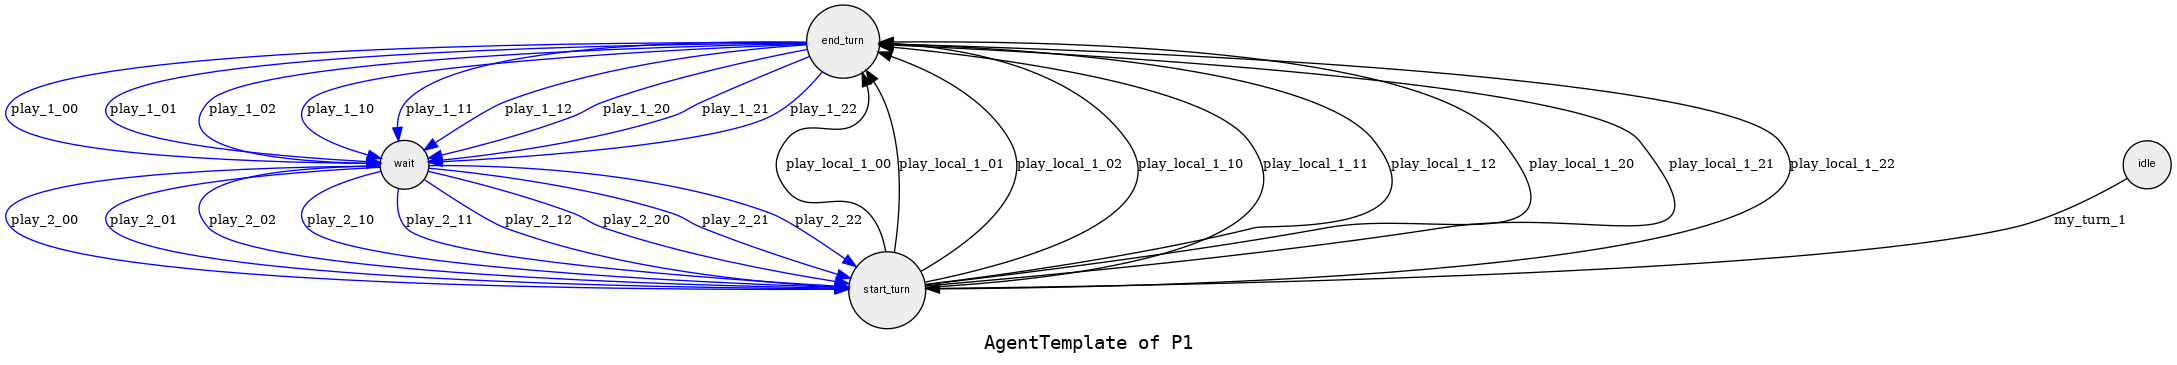
\includegraphics[width=\linewidth]{/home/pawblo/Desktop/future_mgr/text/figures/model-AgentTemplate_P1.png}
  \caption{Model agenta P1}
  \label{fig:enter-label}
\end{figure}

\begin{figure}[h]
  \centering
  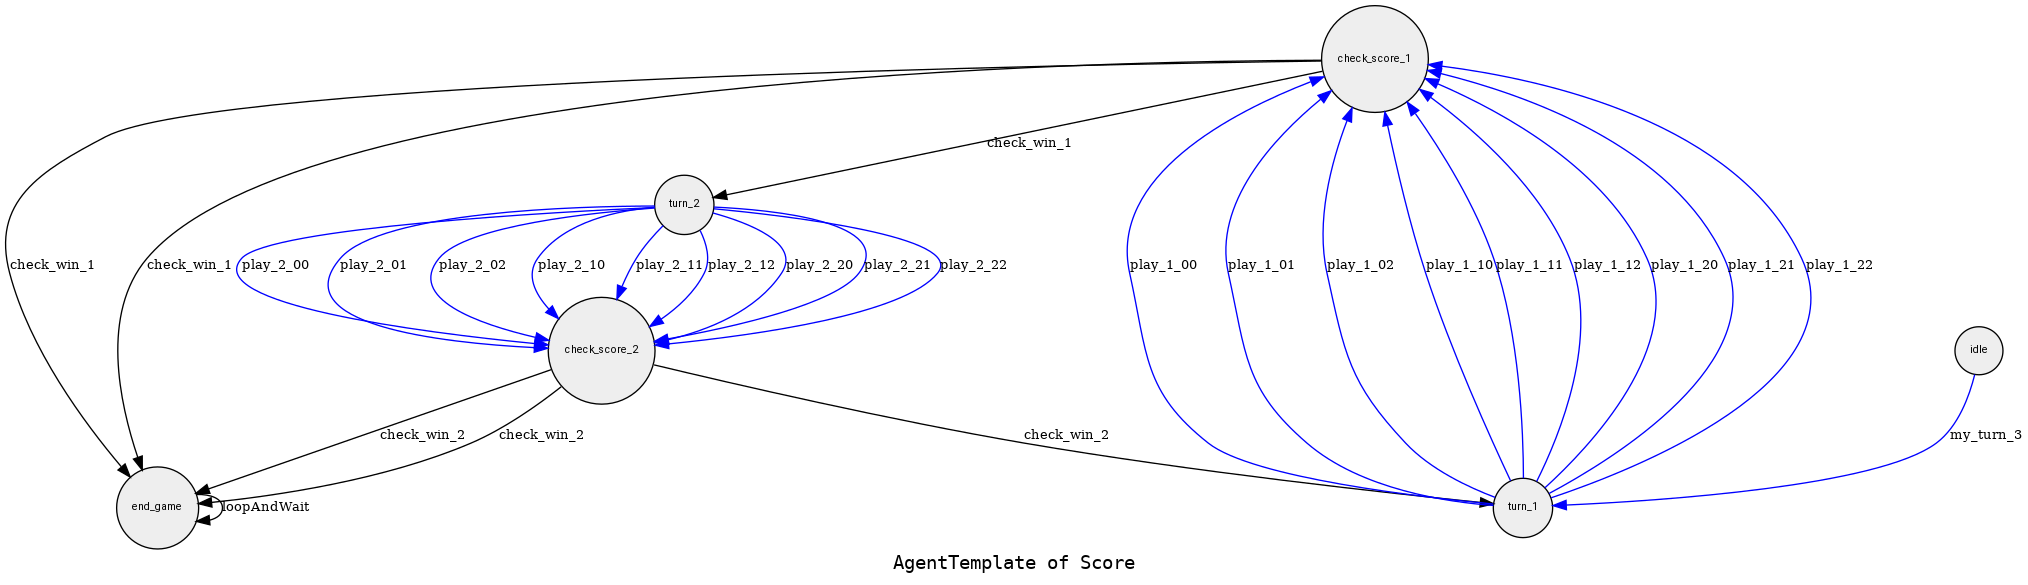
\includegraphics[width=\linewidth]{/home/pawblo/Desktop/future_mgr/text/figures/model-AgentTemplate_Score.png}
  \caption{Model agenta Env}
  \label{fig:enter-label}
\end{figure}


Na grfach możemy sprawdzić czy nasz zaprojektowany model działa tak jak zaplanowaliśmy. Jest to też ważna
funkcjonalnośc w kontekście debugowania i analizy działania modelu. W naszym kontekście możemy przeanalizować, 
czy nasz model zadziała dobrze w kontekście naszej gry w kółko i krzyżyk.



\subsection*{Eksperymenty - STV}
Analizę rozpoczniemy od analizy czasu jakiego potrzebuje \textit{stv} do werfikacji formuły. Pomiary prowadzimy dla gry kółko i krzyżyk 
na planszy o rozmiarach $3 \times 3$.
\begin{table}[h!]
  \centering
  \begin{tabular}{|c|c|c|c|}
  \hline
  Wolne pola & Czas wykonania (s)  \\
  \hline
  1 & 0.007 \\
  2 & 0.01 \\
  3 & 0.01 \\
  4 & 0.02 \\
  5 & 0.07 \\
  6 & 0.45 \\
  7 & 4.35 \\
  8 & 32 \\
  9 & 522\\
  \hline
  \end{tabular}
  \caption{Wyniki checkera stv dla gry na planszy 3x3}
  \label{table:mcmas_results}
  \end{table}
  Dla liczby wolnych pól powyżej $7$ czas werfikacji przekrasza $1s$, dla liczby wolnych $9$ czas wynosi około $10$ minut. Oznacza, to że do werfikacji czy istnieje strategia 
  wygrywająca dla danego gracza w grze kółko i krzyżyk na planszy $3 \times 3$ potrzebny jest czas $10$ minut. 
  Dalej będziemy rozwiązywali to zagadnienie z pomocą uczenie ze wzmocnieniem.

  \subsection*{Uczenie ze wzmocnieniem}
  Celem eksperymentów z użyciem uczenia ze wzmocnieniem jest odpowiedź na pytanie czy istnieja dla graczy 
  strategia wygrywająca dla danej pozycji i gry w czasie istotnie mniejszym niż robi to klasyczny model 
  checker. Wykorzystamy w tym celu trzech różnych agentów - graczy:
  \begin{itemize}
    \item \textit{AlphaZero} 
    \item \textit{MCTS} 
    \item \textit{Random}
  \end{itemize}
  Odpowiednio dwaj pierwszy to gracze wykorzystujący algorytmy o tych samych nazwach, a trzeci agent 
  to agent wykonujący losowe ruchy. Rozpoczniemy od prostego testu rozegrania 
  partii pomiędzy tymi trzem agentami. Rozegramy pomiędzy nimi $100$ partii, 
  odzielnie dla każdej ze stron. Przyjmiemy przy tym domyślne paramtery które w 
  dalszej części zostaną poddane analizie.
  \begin{center}
    \textbf{Tabela wyników rozgrywek pomiędzy graczami}
    \end{center}
  \begin{longtable}{|c|c|c|c|c|c|}
    \hline
    \textbf{Gracz 1} & \textbf{Gracz 2} & \textbf{Wynik} & \textbf{Czas}(s) \\ \hline
    AlphaZero & MCTS & 26:3 & 7.4 \\ \hline
    AlphaZero & Random & 99:0 & 5.8\\ \hline
    MCTS & AlphaZero & 0:0 & 8.7\\ \hline
    MCTS & Random & 97:0 &  5 \\  \hline
    Random & MCTS & 3:80 & 4.7 \\ \hline
    Random & AlphaZero & 0:90 & 6.4 \\ \hline
    \end{longtable}
    Wynik $x:y$ czytamy tak, że Gracz $1$ wygrał $x$ rozgrywek, Gracz $2$ wygrał  $y$ 
    rozgrywek a $100-x-y$ rogrywek zakończyło się remisem. Pierwsza obserwacja 
    jest taka, że byciem graczem rozpoczynającym grę daje pewną przewagę. Widzmy również, 
    że gracz \textit{AlphaZero} nie przegrał całościowo żadnej serii gier. Dla algorytmów 
    \textit{MCMAS} i \textit{AlphaZero} maksymalna liczba symulacji została ustawiona na $100$.

    Zbadamy teraz jak zmienią się wyniki pomiędzy tymi graczami wraz ze zmianą maksymalnej 
    liczby symulacji.

    \begin{longtable}{|c|c|c|c|c|}
      \hline
      \textbf{Gracz 1} & \textbf{Gracz 2} & \textbf{Wynik} & \textbf{Czas} & \textbf{liczba symulacji} \\ \hline
      AlphaZero & MCTS & 33:0 & 6,5 & 50 \\ \hline
      AlphaZero & MCTS & 23:9 & 7,3s & 100 \\ \hline
      AlphaZero & MCTS & 21:6 & 9,8s & 150 \\ \hline
      AlphaZero & MCTS & 10:0 & 12,3s & 200 \\ \hline
      AlphaZero & MCTS & 10:0 & 13,9s & 250 \\ \hline
      AlphaZero & MCTS & 5:0 & 15,3s & 300 \\ \hline
      AlphaZero & MCTS & 8:0 & 16,7s & 350 \\ \hline
      AlphaZero & MCTS & 3:0 & 19,3s & 400 \\ \hline
      AlphaZero & MCTS & 3:0 & 20,0s & 450 \\ \hline
      AlphaZero & MCTS & 6:0 & 21,9s & 500 \\ \hline
      \end{longtable}

    Badanie to pokazuje nam 2 fakty. Pierwszym z nich jest to, że wraz z większeniem liczby symulacji 
    zwiększa się liczba rogrywek remisowych, a przewaga gracza pierwszego w tym przypadku \textit{AlphaZero}
    zmniejsza się. Gdy odwrócimy strony, 
    \begin{longtable}{|c|c|c|c|c|}
      \hline
      \textbf{Gracz 1} & \textbf{Gracz 2} & \textbf{Wynik} & \textbf{Czas} & \textbf{liczba symulacji} \\ \hline
      MCTS & AlphaZero & 21:3 & 8,5s & 50 \\ \hline
      MCTS & AlphaZero & 0:0 & 9,7s & 100 \\ \hline
      MCTS & AlphaZero & 0:1 & 11,4s & 150 \\ \hline
      MCTS & AlphaZero & 1:0 & 12,9s & 200 \\ \hline
      MCTS & AlphaZero & 0:0 & 15,1s & 250 \\ \hline
      MCTS & AlphaZero & 0:0 & 16,s & 300 \\ \hline
      MCTS & AlphaZero & 0:0 & 19,4s & 350 \\ \hline
      MCTS & AlphaZero & 0:0 & 20,3s & 400 \\ \hline
      MCTS & AlphaZero & 4:0 & 21,2s & 450 \\ \hline
      MCTS & AlphaZero & 15:0 & 23,3s & 500 \\ \hline
      \end{longtable}
    Po obróceniu graczy wyniki są zbliżone. Ponownie w środku tabeli mamy 
    bardzo dużo, a właściwie same remisy. Ciekawym zjawiskiem może być 
    zwiększenie liczby wygranych gracz \textit{MCTS} przy dużej liczby symulacji.
    Może to być powodem lepszej i bardziej dokładnej ocenie pozycji 
    poprzez wykonanie dużej liczby symulacji, a model gracza \textit{AlphaZero}
    nie został dotrenowany na takim poziomie, aby był w $100\%$ skuteczny. 
    
    Kolejną krótką analizę przeprowadzimy już od pewnego stanu początkowego 
    zastanego na planszy. Różnica ta nam wprowadzi też pewien nowy element, 
    mianowicie gra nie będzie już grą remisową. Pierwszy gracz w naszej pozycji 
    będzie miał strategię wygrywającą.
    Pozycję którą będziemy analizowali znajdziemy poniżej. Zakładamy, że na ruchu 
    jest gracz \textit{x}.

    \begin{center}
      \begin{tikzpicture}[scale=2]
          % Draw the grid
          \draw (0,0) grid (3,3);
      
          % Add the initial position
          \node at (0.5, 2.5) {\huge X};
          \node at (1.5, 2.5) {\huge O};
          
      \end{tikzpicture}
      \end{center}

      \begin{longtable}{|c|c|c|c|c|}
        \hline
        \textbf{Gracz 1} & \textbf{Gracz 2} & \textbf{Wynik} & \textbf{Czas(s)} & \textbf{liczba symulacji} \\ \hline
        MCTS & AlphaZero & 78:0 & 4,7 & 50 \\ \hline
        MCTS & AlphaZero & 95:0 & 5,4 & 100 \\ \hline
        MCTS & AlphaZero & 96:0 & 5,5 & 150 \\ \hline
        MCTS & AlphaZero & 92:0 & 6,9 & 200 \\ \hline
        MCTS & AlphaZero & 96:0 & 7,6 & 250 \\ \hline
        MCTS & AlphaZero & 94:0 & 7,8 & 300 \\ \hline
        MCTS & AlphaZero & 99:0 & 9,0 & 350 \\ \hline
        MCTS & AlphaZero & 100:0 & 7,1 & 400 \\ \hline
        MCTS & AlphaZero & 100:0 & 6,0 & 450 \\ \hline
        MCTS & AlphaZero & 100:0 & 6,0 & 500 \\ \hline
        \end{longtable}

        \begin{longtable}{|c|c|c|c|c|}
          \hline
          \textbf{Gracz 1} & \textbf{Gracz 2} & \textbf{Wynik} & \textbf{Czas(s)} & \textbf{liczba symulacji} \\ \hline
          AlphaZero & MCTS & 100:0 & 4,9 & 50 \\ \hline
          AlphaZero & MCTS & 1000:0 & 5,0 & 100 \\ \hline
          AlphaZero & MCTS & 100:0 & 5,3 & 150 \\ \hline
          AlphaZero & MCTS & 100:0 & 5,7 & 200 \\ \hline
          AlphaZero & MCTS & 100:0 & 5,9 & 250 \\ \hline
          AlphaZero & MCTS & 100:0 & 6,3 & 300 \\ \hline
          AlphaZero & MCTS & 100:0 & 6,0 & 350 \\ \hline
          AlphaZero & MCTS & 100:0 & 6,4 & 400 \\ \hline
          AlphaZero & MCTS & 100:0 & 6,1 & 450 \\ \hline
          AlphaZero & MCTS & 100:0 & 6,8 & 500 \\ \hline
          \end{longtable}
    Obie tabele dały nam obiecujące wyniki. Widzimy, że liczba gier remisowych 
    jest bardzo mała. Tylko dla liczby symulacji równej $50$ liczba gier remisowcyh 
    była większa niż $10 \%$. Zauważmy dalej, że gracz mająct strategię wygrywającą 
    nigdy nie przegrał rozgrywki. Cofając się do poprzednich tabel w których 
    liczba remisów dla pozycji remisujących wynosiła ponad $70 \%$ widzimy znaczącą 
    różnicę w odsektu remisów w zależności od tego, czy któryś z graczy 
    ma pozycję wygrywającą czy pozycja jest remisująca. To bardzo pozytywne wyniki,
    gdyż potwierdzają one, że wykorzystanie metod uczenia ze wzmocnieniem 
    może być pomocne dla werfikacji pewnych modeli. Może też być szybsze, 
    na aktualnym przykładzie uzyskaliśmy drobne przyspieszenie wynoszące maksylanie 
    $10$ krotność. Eksperyment ten, nie służył uzyskaniu błyskawicznych wyników 
    dla małych modeli. Dla małych modeli narzędzia werfikacji sprawdzają się dobrze.
    Naszym calem było sprawdzenie naszej metody na małym przykładzie aby później 
    z większą pewności i doświadczeniem przetestować ją na większych przykład 
    dla których klasyczne narzędzia werfikacji modelowej nie wystarczają.
          
    Narzędzie \textit{STV} ma swoje ograniczenia czasowe. Sprawdzenie pustej 
    planszy $3 \times 3$ zajmuje około $10 $ minut. Rozegranie $100$ gier 
    i przeprowadzenie po kilkaset symulacji dla naszych algorytmów zajmuje 
    około minuty (czas trwania tranowania \textit{AlphaZero} to $40$s i około 
    $20$ na symulację rozgrywek). Na podstawie tak zebranych danych możemy 
    z dużym prawdopodobieństwem ocenić pozycję jako remisową. Jeśli chcemy 
    przejść na większe plansze jak $5 \times 5$ czy decelowo $5 \times 5 \times 5$,
    musimy zmienić podejście do badania. Ja zdecydowałem na wybór innego narzędzia 
    do dalszych badań. Narzędzia które dłużej istnieje na rynku i ma swoją 
    ugruntowaną pozycję.





\section{Model checker MCMAS}
Gra została zamodelowana w języku \textit{ISPL}. Jest to język który jest wykorzystywany przez narzędzie \textit{MCMAS}.
Przedstawimy kluczowe fragmenty modelu dla lepszego zrozumienia problemu i tego, w jakis posób działa werfikacka modelu.

% Gra została zamodelowana w formacie \textit{ISPL} który obsługuje \textit{MCMAS}. Przedstawione i omówione zostaną 
% kluczowe fragmenty modelu.
% \begin{lstlisting}[language={}]
%     Semantics=SingleAssignment;
%     \end{lstlisting}
%     \textbf{Description}: Specifies the semantics to be used in the model. `SingleAssignment` indicates that variables are assigned values only once per state transition.
    
%     \section{Environment Agent}
    \begin{lstlisting}[language={}]
    Agent Environment
      Obsvars:
        turn : {nought, cross};
        b11 : {x, o, b}; b12 : {x, o, b}; b13 : {x, o, b}; b14 : {x, o, b}; b15 : {x, o, b};
        b21 : {x, o, b}; ... 
       ...
      end Obsvars
    \end{lstlisting}
    Agent \textit{Environment} przechowuje dwa typy zmiennych. Agent posiada zmienną typu \textit{enumerate} czyli typu wyliczanego 
    która przechowuje informację o tym, który z graczy jest aktualnie na ruchu. Kolejne zmienne przechowują informację, o stanie 
    danego pola na planszy. Zmienna $bij$ przechowuje informację na temat pola w i-tym wierszu i -jtej kolumnie. Standard $ISPL$
    nie dopuszcza tablic, dlatego planszę musimy implementować za pomocą $n^{2}$ zmiennych. 
%       Actions = { }; 
%       Protocol: end Protocol
    \begin{lstlisting}[language={}]
      Evolution:
        turn=nought if turn=cross; turn=cross if turn=nought;
        b11 = o if turn = nought and Nought.Action = a11;
        b11 = x if turn = cross  and Cross.Action  = a11;
        ...
        b55 = o if turn = nought and Nought.Action = a44;
        b55 = x if turn = cross  and Cross.Action  = a44;
      end Evolution
    end Agent
     \end{lstlisting}
     Tury graczy zmieniją się na przemian. Agent \textit{Environment} pobiera od agentów graczy akcji jakie podjeli i aktualizuje 
     planszę gry jak i aktualną turę.
%     \textbf{Description}: The \texttt{Environment} agent maintains the game state, including the current turn (\texttt{turn}), and the state of each cell on the 4x4 board (\texttt{b11, b12, ... , b44}). The \texttt{Evolution} section updates the board and turn based on the actions of \texttt{Nought} and \texttt{Cross} agents.
    
    \begin{lstlisting}[language={}]
    Agent Nought
      Vars:
        null : boolean; -- for syntax reasons only
      end Vars
      Actions = {a11,a12,a13,a14,a15,a21,a22,a23,a24,
                a25,a31,a32,a33,a34,a35,a41,a42,a43,a44,a45,a51,a52,a53,a54,a55, };
      Protocol: 
        Environment.b11=b:{a11}; Environment.b12=b:{a12}; ... Environment.b15=b:{a15};
        ...
        Environment.b51=b:{a51};
      end Protocol
    end Agent
    \end{lstlisting}
    Powyżej znajduje się szkic implementacji agenta \textit{Nought}. Implementacja agenta \textit{Cross} jest symetryczna.
    Agent gracza ma do wyboru $n^{2}$ akcji typu $aij$. Każda taka akcja oznacza wykonanie ruchu i postawienie znaku w i-tym wierszu i j-tej kolumnie.
    Akcja taka może zostać wykonana jeśli pole na planszy jest puste.
    \begin{lstlisting}[language={}]
    Evaluation
      noughtwins if
        Environment.b11 = o and Environment.b12 = o and Environment.b13 = o or
        Environment.b14 = o and Environment.b15 = o or 
        ...
        Environment.b11 = o and Environment.b21 = o and Environment.b31 = o or
        Environment.b41 = o and Environment.b51
        ... 
        Environment.b11 = o and Environment.b22 = o and Environment.b33 and 
        Environment.b44 = o and Environment.b55 = o 
    end Evaluation
    \end{lstlisting}
    Sekcja ewaluacji zawiera w sobie warunki na zakończenie gry. Gracz wygrywa jeśli zapełni jedną kolumnę, wiersz 
    lub główną przekątną swoimi znakami. Warunków na zakończenie gry jest $2n+2$. Warunki zakończenia dla obu graczy 
    są takie same, różnią się tylko znakami.
    \begin{lstlisting}[language={}]
        InitStates
  Environment.b11=b and Environment.b12=b and Environment.b13=b 
  and Environment.b14=b and Environment.b15  = b 
  ...
  and Environment.turn = cross
end InitStates
\end{lstlisting}
Sekcja \textit{InitStates} zawiera w sobie stan początkowy modelu. Wszystka pola planszy są puste, a jeden z graczy 
jest graczem startowym.

\begin{lstlisting}[language={}]
Groups
  nought = {Nought}; cross = {Cross};
end Groups

Formulae
  <cross> F (crosswins and ! noughtwins); -- TRUE
  <nought> F (noughtwins and ! crosswins); -- FALSE
end Formulae
\end{lstlisting}
Ostatnim elementem modelu jest zadeklarowanie koalicjii agentów. W naszym przypadku koalcjia agentów składa się z jednego gracza.
Formuły jakie badamy, to formuły które sprawdzają czy dany gracz wygra. Zawsze sprawdzamy dwie formuły, 
aby uzyskać odpowiedź dla każdego z dwóch graczy.
\subsection{Badania}
Analizę wyników zaczniemy od analizy wyników uzyskanych za pomocą narzędzia \textit{MCMAS}.
\begin{table}[h!]
    \centering
    \begin{tabular}{|c|c|c|c|}
    \hline
    Rozmiar planszy & Czas wykonania (s) & Liczba osiągalnych stanów & Użycie pamięci BDD  \\
    \hline
     2x2 &  0.017 &41  & 8.8 MB  \\
     3x3 & 0.325 &6172 & 13.2 MB \\
     4x4&193.383 &1.01786e+07 & 168 MB \\
     5x5 & timeout & timeout & timeout \\
    \hline
    \end{tabular}
    \caption{Wyniki checkera MCMAS}
    \label{table:mcmas_results}
    \end{table}
    Badając rozgrywkę dla pustej planszy $n \times n$ już dla $n=5$ dostajemy timeout.
    Jest to związane wykładniczą eksplozją stanów jakie \textit{MCMAS} ma do przeanalizowania.
    Eksplozja stanów jest bezpośrednio związana z liczbą pól na jakich gracze mogą 
    dokonywać ruchów. Do dalszej analizy wykorzystamy częściowo zapełnioną planszę o rozmiarze 
    $5 \times 5 $ z pozostałymi 17 polami lub więcej.

    \begin{table}[h!]
      \centering
      \begin{tabular}{|c|c|c|c|}
      \hline
      Wolne pola & Czas wykonania (s) & Liczba osiągalnych stanów & Użycie pamięci BDD (MB)  \\
      \hline
      17 &  20.644 & 2.96682e+07  & 49.41   \\
       19 & 199.467 &2.5328e+08 & 125.25 \\
       20& 641.051 &7.4155e+08 & 273.37 \\
       21 & 1714 &2.1736e+09 & 575.39 \\
       22 & 8840 & 6.37789e+09 & 1225\\ 
      \hline
      \end{tabular}
      \caption{Wyniki checkera MCMAS}
      \label{table:mcmas_results}
      \end{table}
      \begin{figure}[h]
        \centering
        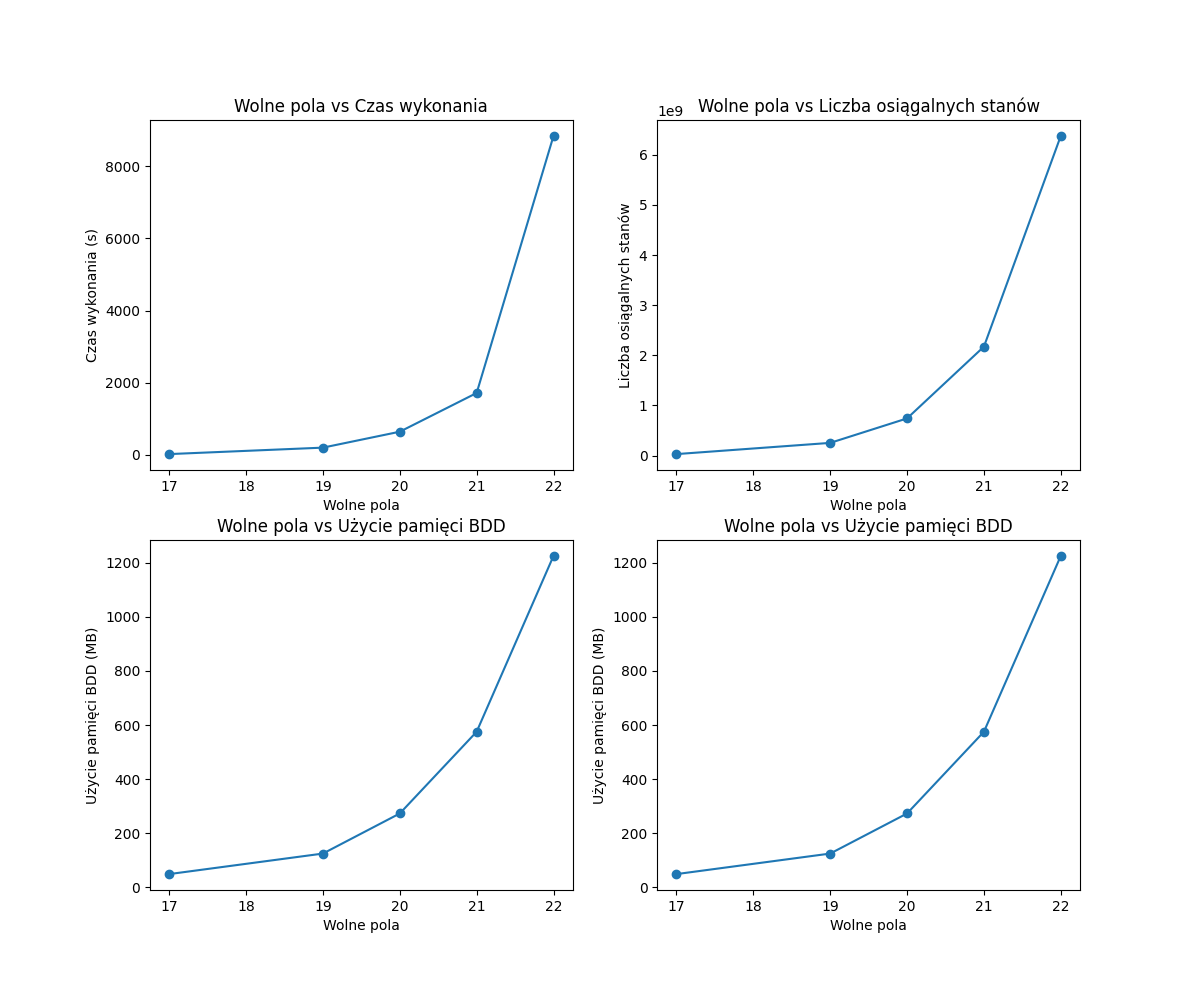
\includegraphics[width=\linewidth]{figures/wykres_wyniki_mcmas_1.png}
        \caption{Wykres wyników dla MCMAS}
        \label{fig:enter-label}
    \end{figure}

Analiza wykresów wskazuje, że czas działania \textit{MCMAS} rośnie 
wykładniczo w stosunku do liczby wolnych pól. 


\chapter{Zakończenie}

Zakończenie pracy zwane również Uwagami końcowymi lub Podsumowaniem powinno zawierać ustosunkowanie
się autora do zadań wskazanych we wstępie do pracy, a w szczególności do celu i zakresu pracy oraz
porównanie ich z faktycznymi wynikami pracy. Podejście takie umożliwia jasne określenie stopnia
realizacji założonych celów oraz zwrócenie uwagi na wyniki osiągnięte przez autora w ramach jego
samodzielnej pracy.

Integralną częścią pracy są również dodatki, aneksy i załączniki zawierające stworzone w ramach pracy programy, aplikacje i projekty.


% \begin{thebibliography}{1}
%     \bibitem{cox}Cox, D. Primes of the Form $x^{2}+ny^{2}$: Fermat, Class Field Theory, and Complex Multiplication. (Wiley,1989)
%     \bibitem{niven}Niven, I., Zuckerman, H. \& Montgomery, H. An Introduction to the Theory of Numbers. (Wiley,1991)
%     \end{thebibliography}

%--------------------------------------
% Literatura
%--------------------------------------

\begin{thebibliography}{1}
   \bibitem{Schlingloff}Schlingloff, B.-H. (2021). Teaching Model Checking via Games and Puzzles. In A. Cerone \& M. Roggenbach (Eds.), Formal Methods - Fun for Everybody (pp. 143-158). Springer International Publishing.
   \bibitem{Gu} Gu, R., Enoiu, E., Seceleanu, C., \& Lundqvist, K. (2020). Verifiable and Scalable Mission-Plan Synthesis for Autonomous Agents. In M. H. ter Beek \& D. Ničković (Eds.), Formal Methods for Industrial Critical Systems (pp. 73-92). Springer International Publishing.
   \bibitem{Amazon} Chong, N., Cook, B., Kallas, K., Khazem, K., Monteiro, F. R., Schwartz-Narbonne, D., Tasiran, S., Tautschnig, M., \& Tuttle, M. R. (2020). Code-level model checking in the software development workflow. Proceedings of the ACM/IEEE 42nd International Conference on Software Engineering: Software Engineering in Practice, 11-20. https://doi.org/10.1145/3377813.3381347   
   \bibitem{Github} GitHub. (2023). The State of Open Source and AI. https://github.blog/2023-11-08-the-state-of-open-source-and-ai/
   \bibitem{Jamroga} Jamroga, W. (2015). Logical Methods for Specification and Verification of Multi-Agent Systems. ICS PAS Publishing House.
   \bibitem{batog1994podstawy}Batóg, T. Podstawy logiki. (Wydaw. Naukowe UAM,1994)
   \bibitem{Deepa}Deepa, R., Velnath, R., Manojkumar, P. \& Mohanraj, K. Artificial Neural Network-Based Tic-Tac-Toe Game. {\em Proceedings Of International Conference On Communication And Computational Technologies }. pp. 55-65 (2023)
   \bibitem{Dalffa2019-DALTLU}Dalffa, M., Abu-Nasser, B. \& Abu-Naser, S. Tic-Tac-Toe Learning Using Artificial Neural Networks. {\em International Journal Of Engineering And Information Systems (IJEAIS)}. \textbf{3}, 9-19 (2019)
   \bibitem{Fogel}Fogel, D. Using evolutionary programing to create neural networks that are capable of playing tic-tac-toe. {\em IEEE International Conference On Neural Networks}. pp. 875-880 vol.2 (1993)
   \bibitem{beck2008combinatorial}Beck, J. Combinatorial Games: Tic-Tac-Toe Theory. (Cambridge University Press,2008)
   \bibitem{sutton1998reinforcement}Sutton, R. \& Barto, A. Reinforcement Learning: An Introduction. (MIT Press,1998)
   \bibitem{alpha_zero}Silver, D., Hubert, T., Schrittwieser, J., Antonoglou, I., Lai, M., Guez, A., Lanctot, M., Sifre, L., Kumaran, D., Graepel, T. \& Others Mastering chess and shogi by self-play with a general reinforcement learning algorithm. {\em ArXiv Preprint ArXiv:1712.01815}. (2017)
   \bibitem{jamroga_stv}Kamiński, M., Kurpiewski, D. \& Jamroga, W. STV+KH: Towards Practical Verification of Strategic Ability for Knowledge and Information Flow. {\em Proceedings Of The 23rd International Conference On Autonomous Agents And Multiagent Systems}. pp. 2812-2814 (2024)
\end{thebibliography}

%--------------------------------------
% Dodatki
%--------------------------------------

\cleardoublepage\appendix%
\newpage
\input{chapters/zalacznik.tex}

%--------------------------------------
% Informacja o prawach autorskich
%--------------------------------------

\ppcolophon

\end{document}
